% This file contains things removed from the analysis chapter on 2023-08-24 or thereabouts
% that I think belongs in the methods chapter.

\begin{figure}
  \centering
  \begin{subfigure}[htpb]{0.9\textwidth}
   \centering
   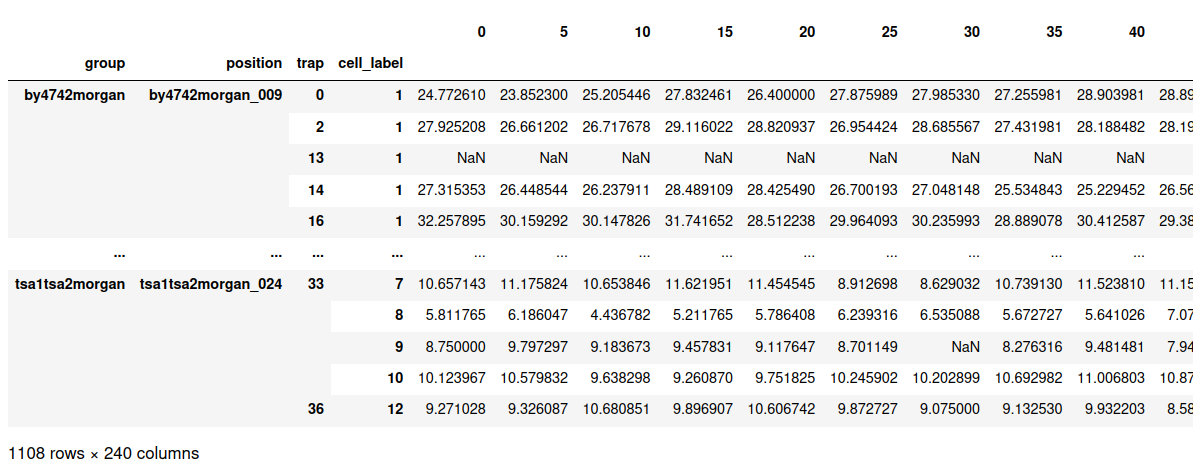
\includegraphics[width=\textwidth]{example_dataframe}
   \caption{
     Example dataframe
   }
   \label{fig:analysis-example-dataframe}
  \end{subfigure}
  \begin{subfigure}[htpb]{0.5\textwidth}
   \centering
   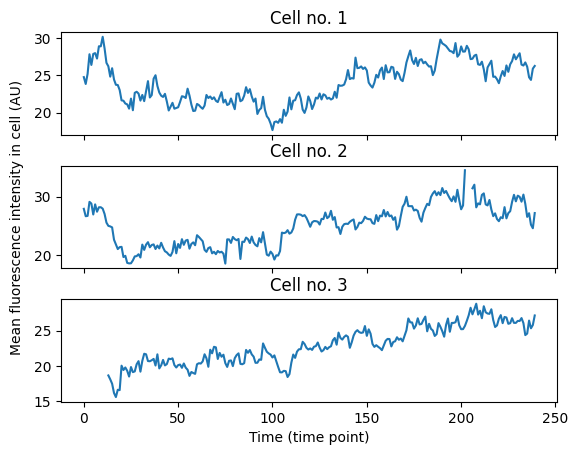
\includegraphics[width=\textwidth]{example_timeseries}
   \caption{
     Example time series
   }
   \label{fig:analysis-example-timeseries}
  \end{subfigure}
  \begin{subfigure}[htpb]{0.5\textwidth}
   \centering
   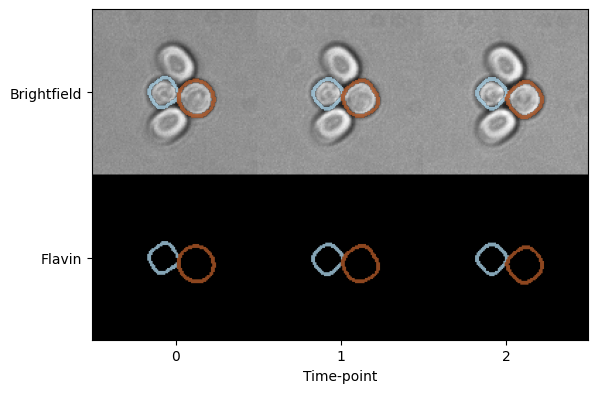
\includegraphics[width=\textwidth]{example_images}
   \caption{
     Example images
   }
   \label{fig:analysis-example-images}
  \end{subfigure}
  \caption[
    Data overview
  ]{
    Data overview.
    The segmentation \& data analysis software \textit{aliby} (see section~\ref{sec:methods-segmentation}) produces a dataframe for each fluorescence channel --- \ref{fig:analysis-example-dataframe} shows the flavin signals for one particular experiment.
    Each row represents a cell and each column represents a time point.
    To illustrate the flavin signals, some sample time series are plotted from the dataframe in \ref{fig:analysis-example-timeseries} --- here, the horizontal axis shows time and the vertical axis shows the mean intensity of the signal in the cell, represented as numbers in the dataframe.
    Each data point derives from images, examples in \ref{fig:analysis-example-images}.
    As discussed in section~\ref{sec:methods-segmentation},
    image segmentation uses the brightfield images to define cell outlines, then \textit{aliby} overlays the cell outlines onto the fluorescent images to extract fluorescence intensity.
    Specifically, this intensity is the mean intensity of pixels within the cell outline, subtracted by the background intensity, and is thus the numerical values represented in each data element in the dataframe.
  }
  \label{fig:analysis-data-overview}
\end{figure}
